\documentclass{article}
\usepackage{tikz}

\begin{document}

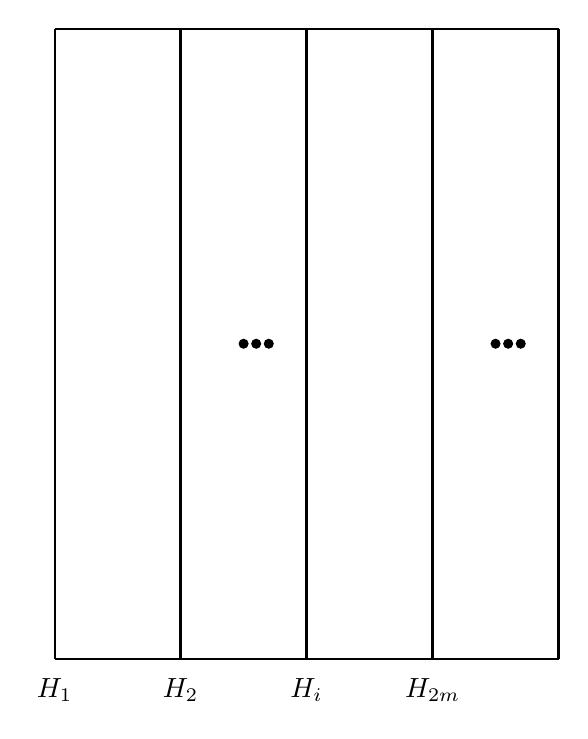
\begin{tikzpicture}[scale=0.8]
    % Draw the vertical lines
    \draw[thick] (0,0) -- (0,10);
    \draw[thick] (2,0) -- (2,10);
    \draw[thick] (4,0) -- (4,10);
    \draw[thick] (6,0) -- (6,10);
    \draw[thick] (8,0) -- (8,10);

    % Draw the horizontal lines
    \draw[thick] (0,0) -- (8,0);
    \draw[thick] (0,10) -- (8,10);

    % Add dots to represent the ellipsis
    \filldraw[black] (3,5) circle (2pt);
    \filldraw[black] (3.2,5) circle (2pt);
    \filldraw[black] (3.4,5) circle (2pt);

    \filldraw[black] (7,5) circle (2pt);
    \filldraw[black] (7.2,5) circle (2pt);
    \filldraw[black] (7.4,5) circle (2pt);

    % Add labels below the lines
    \node at (0,-0.5) {$H_{1}$};
    \node at (2,-0.5) {$H_{2}$};
    \node at (4,-0.5) {$H_{i}$};
    \node at (6,-0.5) {$H_{2m}$};
\end{tikzpicture}

\end{document}